\chapter{Bluetooth Stack Implementation}
\label{chp:btstackimp}
\lhead{Chapter \ref{chp:btstackimp}. \emph{Bluetooth Stack Implementation}}

The development of the Bluetooth stack followed a bottom-up development methodology, designing and writing each software layer in sequence from the lowest layer first, to the highest and most abstracted layers last. This sequence ensured that each layer was functionally correct and could be verified before the higher layers were implemented. This suited the development of the Bluetooth stack---and, indeed, most software stacks---as each higher software layer is dependant solely on lower logical layers in the stack.

\section{Software Overview}

The software layers implemented in the completed Bluetooth stack are shown in Figure \ref{fig:completedbtstacklayers}.

\begin{figure}[tbph]
	\vspace{1em}
	\centering
		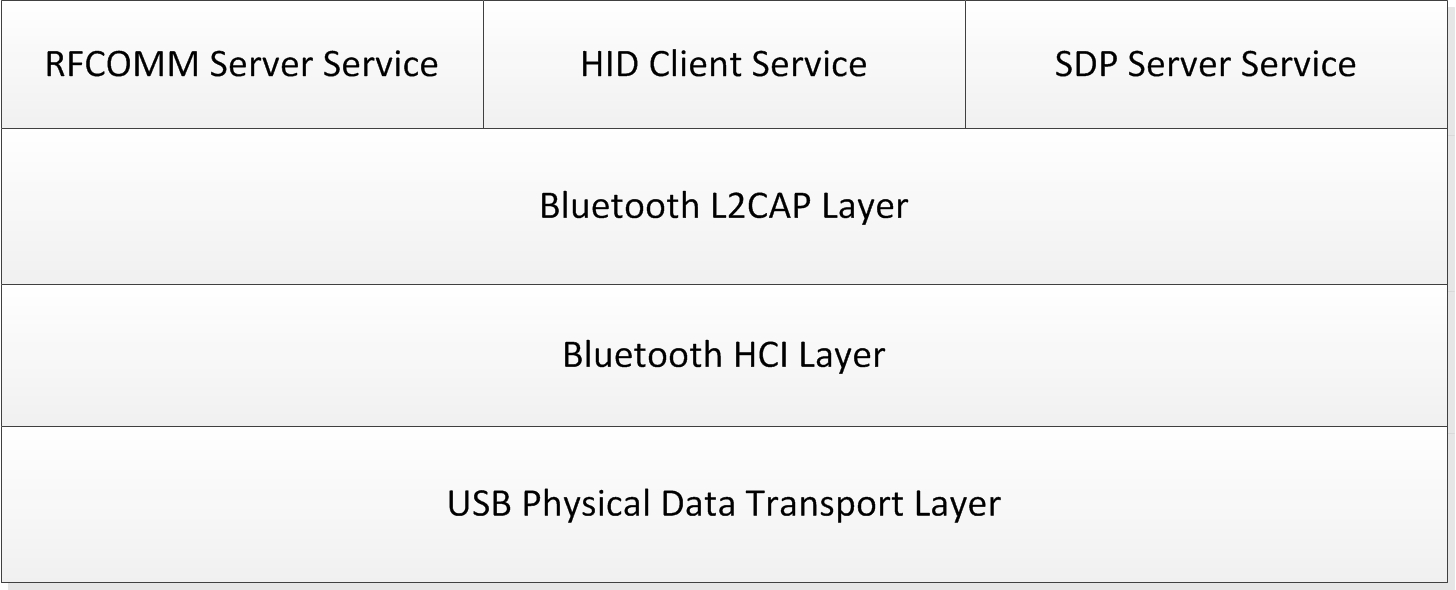
\includegraphics[width=100mm]{CompletedBluetoothStack.png}
	\rule{35em}{0.5pt}
	\caption[Diagram of the completed Bluetooth stack layers]{Diagram showing the completed layers of the Bluetooth stack.}
	\label{fig:completedbtstacklayers}
\end{figure}

% TODO

\section{Design Restrictions}

A number of design restrictions were placed on the development of the Bluetooth stack; these ensured that the completed stack remained modular, extensible and suitable for integration in a wide range of embedded systems with various capabilities, and conversely, limitations. As an unfortunate but expected side effect, a number of these restrictions complicated the software development process significantly.

\FloatBarrier
\subsection{No Heap Memory Allocations}

The largest restriction placed on the stack design was the requirement of static and stack allocated memory allocation only --- no dynamic heap allocated memory was to be used via the usual \lstinline{malloc()} and \lstinline{free()} functions from the \texttt{libc} library. Most embedded environments contain three types of memory allocations:

\begin{enumerate}
	\item \textbf{Static Allocations}, including global variables and \lstinline{static} qualified variables.
	\item \textbf{Stack Allocations}, automatically populated to store local automatic variables, function paramaters, return addresses, etc.
	\item \textbf{Heap Allocations}, persistant dynamic allocations manually managed by the user application.
\end{enumerate}

However, for significantly memory constrained systems, heap allocations are generally avoided due to the possibility of memory fragmentation; large numbers of differently-sized allocations and deallocations may cause fragmented holes to appear within the heap environment, causing allocation exhaustion to occur even if sufficient (raw) memory is available for an allocation request. In addition, dynamic memory complicates the formal analysis of a program, making memory requirements harder to judge, and thus harder to determine whether a given set of firmware will operate correctly within a specified environment without further in-depth analysis. In large embedded environments (ones with virtual memory management, and/or a large heap space) these problems are less of an issue and dynamic memory may be preferable for its simplicity.

The design of embedded stacks based on a no-heap-allocation strategy is a complex one, requiring certain trade-offs to be made. In the case of the Bluetooth stack presented here, a major side-effect of this decision was the need to fix the maximum number of simultaneous HCI device connections, L2CAP channel connections, and other queue- and list-like data structures within each instance of the stack. A major downside to this approach is the increased complexity of packet buffering and re-assembly, as fixed-size buffers must be used.

\FloatBarrier
\subsection{Endianness Correction}

A second complication based on the physical constraints from the execution environment is the native endianness of the processor hardware, i.e., the order in which multiple-byte data values are stored inside the processor. Depending on the execution architecture, data values may be represented in Big Endian (most significant byte at the lowest address) or Little Endian (least significant byte at the lowest address) format within the CPU. Data transmitted and received at the local device to remote device boundary must undergo a encoding conversion if the endianness of the source and sink do not match.

In the case of the Bluetooth specification, this was further complicated by the various layers; some layers used Little Endian encoding for exchanged data, while others selected Big Endian. To perform the correct encoding/decoding on each platform, a set of conversion macros were implemented at points where multi-byte values were exchanged. This ensured that regardless of the native endian format of the architecture the stack is compiled to, multi-byte values will be interpreted correctly.

\FloatBarrier
\subsection{Physical Transport Independance}

% TODO

\FloatBarrier
\subsection{Bluetooth Specification Compatibility}

For a software stack to be suitable for general use, it must be designed around, and undergo a series of tests to ensure compatibility with, a particular version of the protocol specification. 

% TODO

\FloatBarrier
\subsection{Multiple Instances, Connections and Channels}

% TODO

\FloatBarrier
\subsection{Minimal Memory Usage}

% TODO

\section{Software Layer Implementation}

% TODO

\FloatBarrier
\subsection{Physical Transport}

% TODO

\FloatBarrier
\subsection{HCI Layer}

% TODO

\FloatBarrier
\subsection{L2CAP Layer}

% TODO

\FloatBarrier
\subsection{Bluetooth Services}

% TODO

\FloatBarrier
\subsubsection{SDP Service}

% TODO

\FloatBarrier
\subsubsection{HID Service}

% TODO

\FloatBarrier
\subsubsection{RFCOMM Service}

% TODO

\section{Integration into User Applications}

% TODO

\FloatBarrier
\subsection{Events and Callbacks}

\begin{figure}[tbph]
	\vspace{1em}
	\centering
		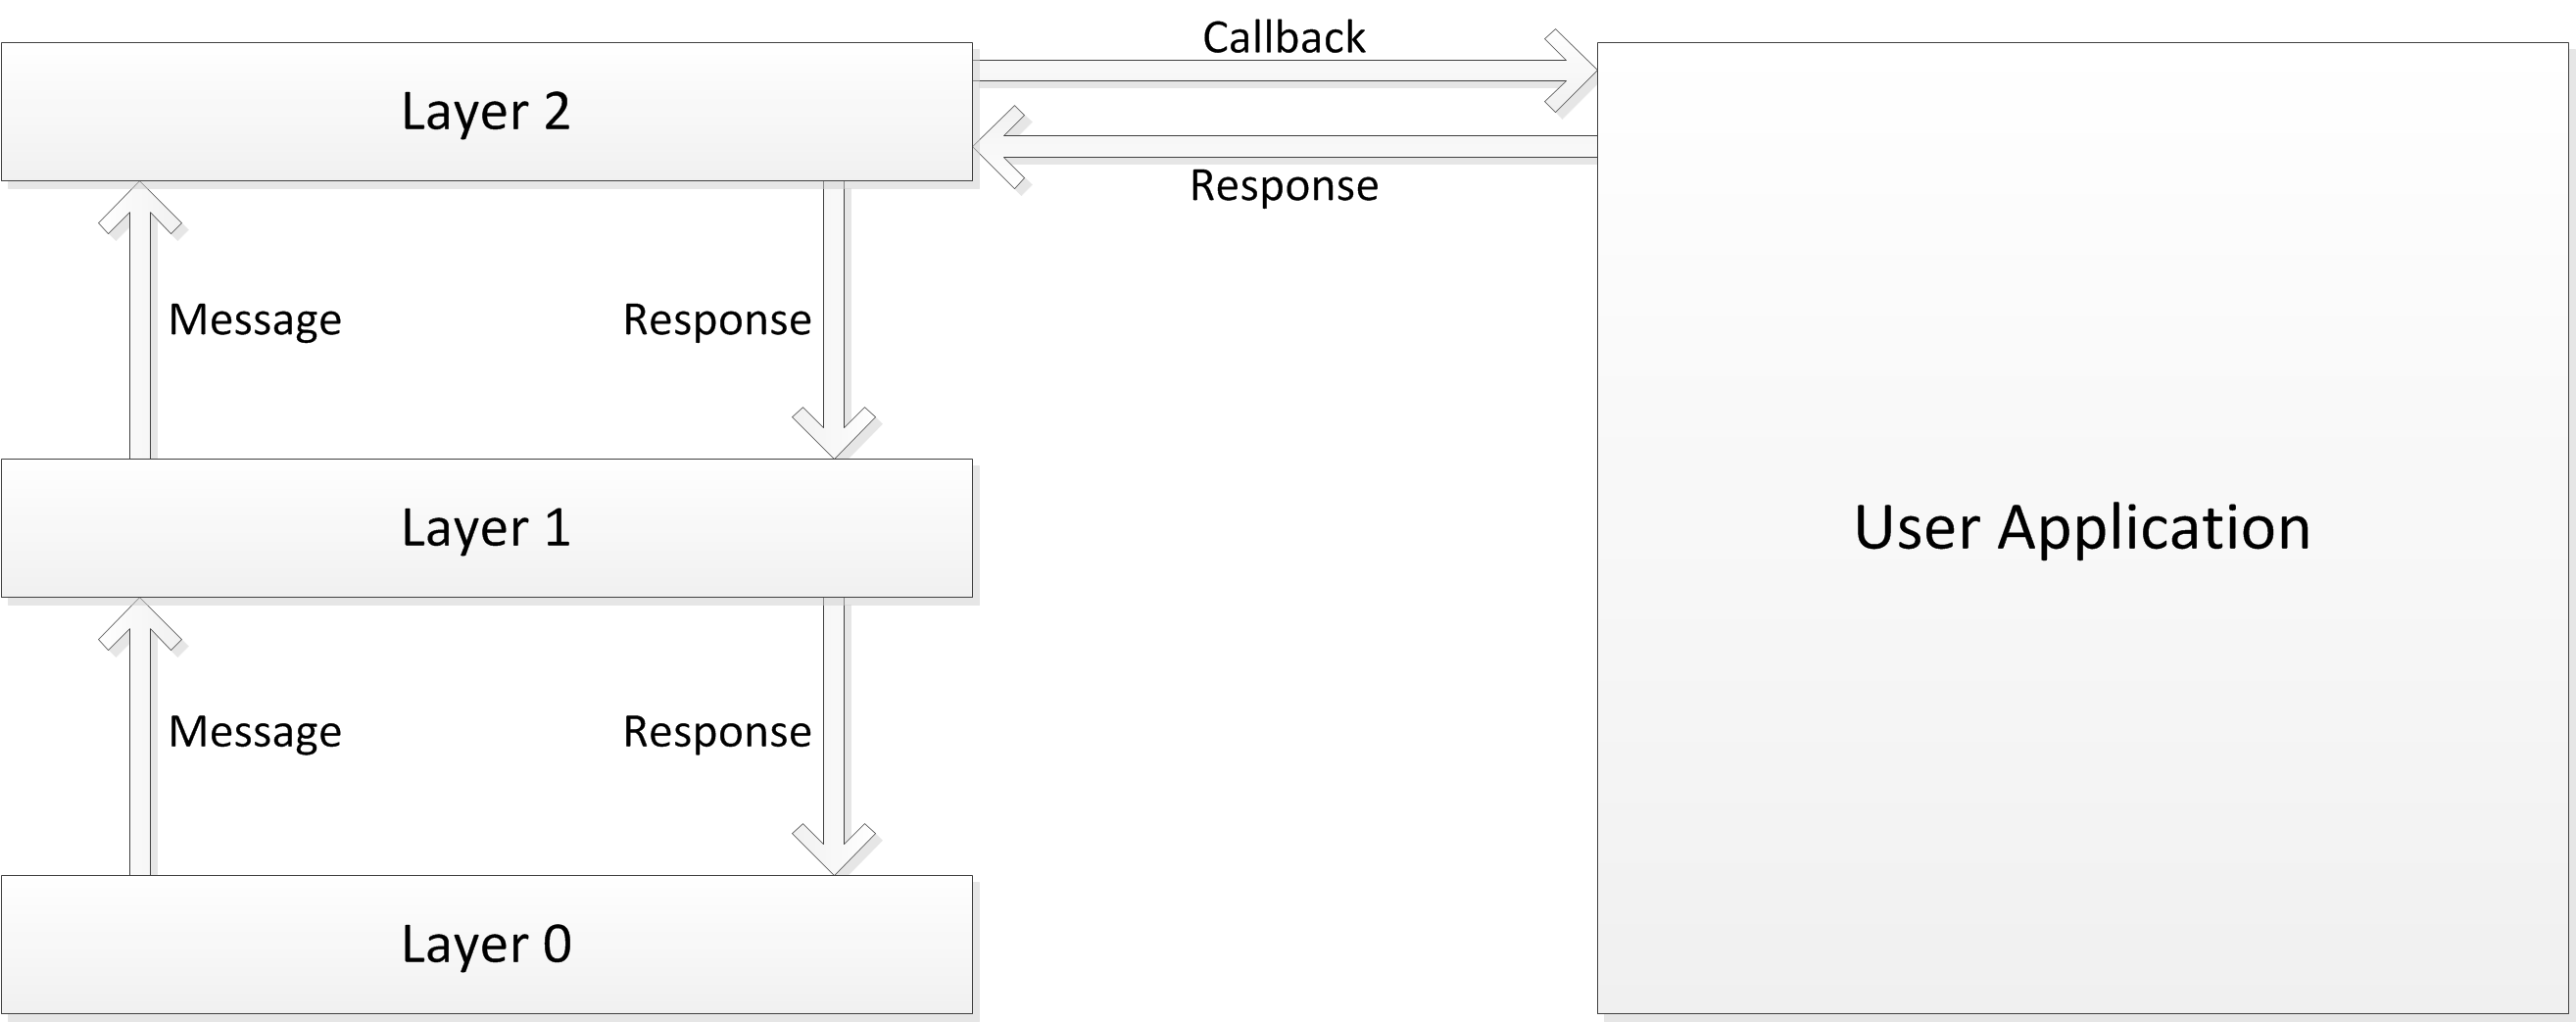
\includegraphics[width=140mm]{MessageResponseCallback.png}
	\rule{35em}{0.5pt}
	\caption[Diagram of the Message, Response and Callback sequence]{Diagram showing the Message, Response and Callback sequence of a typical software stack when passing a message and response through several intermediate layers.}
	\label{fig:messageresponsecallback}
\end{figure}

% TODO

\FloatBarrier
\subsection{Management Functions}

% TODO